\documentclass[12pt,a4paper]{article}

%%%%%%% INFORMAÇÕES DO CABEÇALHO
\newcommand{\workingDate}{\today}

%% Pacotes essenciais
\usepackage[utf8]{inputenc}
\usepackage[T1]{fontenc}
\usepackage[brazil]{babel}
\usepackage[a4paper,margin=2.5cm]{geometry}
\usepackage{microtype}

%% Pacotes adicionais
\usepackage{booktabs}
\usepackage{array}
\usepackage{multirow}
\usepackage{enumitem}
\usepackage{xcolor}
\usepackage{tikz}
\usepackage{float}
\usepackage{graphicx}
\usepackage{fancyhdr}
\usepackage{listings}
\usepackage{caption}
\usetikzlibrary{shapes.geometric, arrows, positioning, fit}

\usepackage{longtable}
\usepackage{colortbl}

%% Configuração de listings para código
\definecolor{codebg}{RGB}{248,248,248}
\definecolor{codeframe}{RGB}{220,220,220}
\definecolor{codecomment}{RGB}{106,153,85}
\definecolor{codestring}{RGB}{206,145,120}
\definecolor{codekeyword}{RGB}{86,156,214}
\definecolor{utfprYellow}{RGB}{255,204,0}
\definecolor{lightGray}{RGB}{245,245,245}
\definecolor{verdeEscuro}{RGB}{31,63,43}
\definecolor{corAtraso}{RGB}{176,58,46}

\lstdefinestyle{webcode}{
    backgroundcolor=\color{codebg},
    frame=single,
    rulecolor=\color{codeframe},
    basicstyle=\ttfamily\small,
    commentstyle=\color{codecomment},
    stringstyle=\color{codestring},
    keywordstyle=\color{codekeyword},
    breaklines=true,
    breakatwhitespace=true,
    tabsize=4,
    showstringspaces=false,
    captionpos=b,
    numbers=left,
    numberstyle=\tiny\color{gray},
    numbersep=5pt,
    xleftmargin=15pt,
    extendedchars=true,
    inputencoding=utf8,
    literate={á}{{\'a}}1 {é}{{\'e}}1 {í}{{\'i}}1 {ó}{{\'o}}1 {ú}{{\'u}}1
             {â}{{\^a}}1 {ê}{{\^e}}1 {ô}{{\^o}}1
             {ã}{{\~a}}1 {õ}{{\~o}}1
             {ç}{{\c{c}}}1 {À}{{\`A}}1 {Á}{{\'A}}1
             {ã}{{\~a}}1 {Ã}{{\~A}}1
}

\lstset{style=webcode}

%% Bibliografia
\usepackage[backend=biber]{biblatex}
\addbibresource{referencias.bib}

%% Cabeçalho com logo
\pagestyle{fancy}
\fancyhf{}
\fancyhead[L]{
\includegraphics[height=1cm]{logo_utf.png}}
\fancyhead[C]{\small\textsc{Relatório Técnico Final do Projeto}}
\fancyhead[R]{\small\textbf{Padrões Web}}
\renewcommand{\headrulewidth}{0.4pt}
\fancyfoot[L]{\small UTFPR -- Curitiba}
\fancyfoot[C]{\small\textit{Última modificação: \today}}
\fancyfoot[R]{\small\thepage}
\renewcommand{\footrulewidth}{0.4pt}

\begin{document}

%% ─── CAPA ────────────────────────────────────────────────────────────────────
\begin{center}
    {\textbf{\huge Relatório Técnico Final}}\\[2mm]
    {\large \textit{Projeto: Influência da Globalização no Vocabulário Brasileiro}}\\[2mm]
    {\normalsize Entrega 3 -- Versão Final}\\[6mm]
    {\normalsize
        \begin{tabular}{rl}
            \textbf{Integrantes:} & Beatriz Fernandes\\
                                  & Gustavo Machado \\
                                  & Johnny Sarafim\\
                                  & Julio Cesar Navas \\
                                  & Thiago Honório \\[3mm]
            \textbf{Disciplina:}  & Padrões Web \\
            \textbf{Curso:}       & Sistemas de informação\\
            \textbf{Campus:}      & UTFPR - Curitiba \\
        \end{tabular}
    }\\[6mm]
    \today
\end{center}

\vspace{4mm}
\hrule height 1pt
\vspace{6mm}

% ─── LICENÇA ─────────────────────────────────────────────────────────────────
{\small
\noindent\textbf{Licença de uso:} Este documento é disponibilizado sob a licença
\textbf{Creative Commons Atribuição 4.0 Internacional (CC BY 4.0)}.
É permitido copiar, distribuir e adaptar o material para qualquer finalidade,
mesmo comercial, desde que seja atribuído o devido crédito aos autores.
Mais informações em: \texttt{https://creativecommons.org/licenses/by/4.0/deed.pt\_BR}.
}

\vspace{6mm}

% ─── RESUMO ──────────────────────────────────────────────────────────────────
\section{Resumo}

Este documento descreve a organização da equipe e o resultado final do desenvolvimento do
projeto \textit{``Influência da Globalização no Vocabulário Brasileiro''}, um site que explora
como termos estrangeiros, especialmente do inglês, foram incorporados ao cotidiano do português
falado no Brasil, a exemplo de palavras como \textit{like}, \textit{story}, \textit{hype} e
\textit{aura}. O documento apresenta o tema e os objetivos do projeto, os papéis exercidos por
cada integrante ao longo do semestre, o modelo de processo de desenvolvimento adotado e o grau
de aderência real ao cronograma planejado, a estrutura final de páginas do site com a descrição
de seus elementos e comportamentos, o modelo de layout CSS utilizado, evidências de código e
imagens que demonstram o atendimento dos objetivos propostos, e as considerações finais sobre o
trabalho realizado.

% ─── OBJETIVOS DO PROJETO ──────────────────────────────────────────────────
\section{Tema e Objetivos do Projeto}

O projeto busca investigar a metamorfose linguística brasileira sob a ótica da globalização
digital. O foco central é compreender como a exposição contínua a conteúdos estrangeiros e a
comunicação em redes sociais moldam o vocabulário das novas gerações.

\subsection{Objetivos quanto ao Tema}
\begin{itemize}[leftmargin=*]
    \item \textbf{Análise de Impacto:} Avaliar como a digitalização crescente atua como vetor
    para a adoção de estrangeirismos e gírias de nicho.
    \item \textbf{Reflexão Crítica:} Debater se essa influência é puramente enriquecedora ou se
    acarreta prejuízos, como o empobrecimento do vocabulário nativo ou dificuldades de
    comunicação intergeracional.
    \item \textbf{Resgate Histórico:} Rastrear a origem e a evolução de termos que hoje são
    onipresentes no cotidiano digital.
\end{itemize}

\subsection{Justificativa da Escolha do Tema}
A escolha deste tema justifica-se pela velocidade sem precedentes com que o português brasileiro
absorve termos globais. Este fenômeno não é apenas linguístico, mas social: entender se essa
tendência é maléfica ou natural é essencial para compreender a identidade da juventude atual. O
projeto se propõe a ser um ponto de equilíbrio entre o registro dessas mudanças e a análise
crítica de seus efeitos na escrita e na norma culta.

% ─── IMPLEMENTAÇÃO DOS OBJETIVOS ─────────────────────────────────────────────
\section{Descritivo de Atendimento dos Objetivos}
\label{sec:descritivo-objetivos}

Para garantir que os objetivos teóricos fossem transpostos para o produto final, as metas foram
atendidas através das seguintes frentes no website, todas concluídas e funcionais nesta entrega
final:

\begin{enumerate}[leftmargin=*, label=\roman*.]
    \item \textbf{Educação e Contexto:} através da \textit{Contextualização do Vocabulário} e da
    \textit{Linha do Tempo}, o usuário compreende que a globalização não é estática,
    identificando as rotas de entrada de novos termos. A página de Contextualização recebeu,
    nesta entrega final, o vídeo explicativo incorporado e a nuvem de palavras interativa
    finalizada, com algoritmo próprio de posicionamento (Seção~\ref{sec:protótipos-contexto} e
    exemplo de código na Seção~\ref{sec:exemplo-nuvem}).
    \item \textbf{Interatividade:} o \textit{Quiz dos Vocabulários} serve como
    ferramenta de aferição de conhecimento, permitindo que o usuário teste seu nível de imersão
    na cultura digital atual. A lógica do quiz foi finalizada nesta entrega, com renderização de
    alternativas, confirmação por questão, bloqueio de resposta após confirmação e tela de
    resultado (Seção~\ref{sec:exemplo-quiz}).
    \item \textbf{Ponte Geracional:} a \textit{Tabela de Tradução} (Dicionário de Gírias) atua
    diretamente na mitigação do hiato comunicativo entre diferentes faixas etárias, traduzindo o
    ``internetês'' para formas de expressão tradicionais, por meio de um dicionário interativo
    com mais de 100 termos, busca em tempo real e paginação animada.
    \item \textbf{Convite à Exploração:} a \textit{Página Inicial} passou a apresentar, nesta
    entrega, \textit{cards} com pré-visualização (\textit{preview}) das demais páginas do site ao
    passar o mouse, facilitando a navegação e dando ao visitante uma antecipação visual do
    conteúdo de cada seção antes mesmo de acessá-la (Seção~\ref{sec:protótipos-home}).
    \item \textbf{Análise de Risco e Benefício:} a página \textit{Impacto nas Gerações} é o
    núcleo dissertativo do projeto. Nesta entrega final, o texto definitivo sobre os possíveis
    malefícios da digitalização em massa (como o declínio da formalidade excessiva) e os
    benefícios (como a agilidade e a universalização da comunicação) foi redigido e incorporado,
    junto a um bloco de dados estatísticos com referências (Seção~\ref{sec:protótipos-impacto}).
\end{enumerate}

% ─── MEMBROS ─────────────────────────────────────────────────────────────────
\section{Membros da Equipe}

A equipe é composta por cinco integrantes, conforme apresentado na Tabela~\ref{tab:membros}. Os
papéis iniciais, atribuídos no começo do projeto, foram utilizados como ponto de partida; a forma
como cada integrante efetivamente atuou ao longo de todo o semestre é detalhada na
Seção~\ref{sec:papeis-semestre}.

\begin{table}[H]
\centering
\caption{Membros da equipe e papéis iniciais.}
\label{tab:membros}
\renewcommand{\arraystretch}{1.4}
\begin{tabular}{>{\centering\bfseries}m{0.5cm} >{\raggedright}m{4.5cm} >{\raggedright\arraybackslash}m{7.5cm}}
\toprule
\textbf{\#} & \textbf{Integrante} & \textbf{Papel inicial} \\
\midrule
1 & Beatriz Fernandes & Desenvolvimento front-end  \\
2 & Gustavo Machado & Criação de conteúdo e revisão de textos e desenvolvedor front-end \\
3 & Johnny Sarafim & Projeto do site e identidade visual e desenvolvedor front-end \\
4 & Julio Cesar Navas & Desenvolvimento front-end \\
5 & Thiago Honório & Teste de funcionalidades e integração de conteúdo e desenvolvedor front-end \\
\bottomrule
\end{tabular}
\end{table}

% ─── PAPÉIS AO LONGO DO SEMESTRE ──────────────────────────────────────────────
\section{Organização do Grupo: Papéis ao Longo do Semestre}
\label{sec:papeis-semestre}

Diferentemente de uma divisão estática de funções, a equipe optou por uma organização
colaborativa em que todos os integrantes atuaram como desenvolvedores front-end, com uma
área de maior concentração de esforço para cada um, que se consolidou ao longo das sprints. A
seguir, descreve-se o papel efetivamente exercido por cada integrante durante o semestre,
incluindo as atividades da fase final de desenvolvimento.

\subsection{Beatriz Fernandes}
Atuou como integrante da equipe de desenvolvimento, com foco na parte de Front-End através do uso de HTML e CSS. Sua participação foi importante para ajudar a construir a identidade visual do website, garantindo a organização do conteúdo, a usabilidade das interfaces e a harmonia visual entre as páginas. No desenvolvimento técnico, colaborou diretamente na criação e implementação das páginas “Página Inicial” e “Contextualização”, trabalhando na estruturação dos textos, na estilização dos elementos e na formatação estética dessas seções.
Além disso, atuou junto aos demais membros do grupo no suporte ao design geral do site, auxiliando em ajustes de layout, correções em CSS e na padronização visual. Também contribuiu com a edição de vídeo do projeto, ajudando a complementar a apresentação do conteúdo. Dessa forma, colaborou para que o site mantivesse uma navegação consistente, fluida e visualmente coesa entre todas as páginas.

\subsection{Gustavo Machado}
Atuou como desenvolvedor Full Stack e redator, como front-end cuidando principalmente do HTML inicial da pagina de contextualização e o HTML/CSS, da pagina sobre, assim como revisão da identidade geral do site. No JavaScript se destaca desenvolvendo da lógica da nuvem de palavras interativa com
um algoritmo de \textit{hash} determinístico para estabilizar visualmente a posição das palavras
entre renderizações e um sistema de detecção de colisão entre caixas de texto, além do mecanismo
de atualização de pesos visuais conforme o usuário insere novos termos.
Como redator, atuou como o escritor principal do relatorio, criando a estrutura, estabelecendo o formato e os tópicos obrigatórios.

\subsection{Johnny Sarafim}
Atuou como Desenvolvedor Full Stack do projeto, no Front-End (HTML, CSS e JavaScript) e no Back-End (JavaScript), além de exercer o papel de Scrum Master e de responsável pela arquitetura geral do website. Sua atuação foi essencial para transformar os objetivos do trabalho em uma solução web organizada, funcional e coerente com a proposta acadêmica.
No desenvolvimento técnico, foi o principal responsável pelas páginas “Página Inicial”, “Linha do Tempo”, “Dicionário de Gírias” e “Impacto no Vocabulário”, cuidando tanto da estrutura visual quanto da lógica de interação e integração entre os componentes. Também contribuiu, em menor escala, com as demais páginas, garantindo padronização de layout, consistência na navegação e unidade na experiência do usuário.
Como Scrum Master, apoiou a equipe no planejamento e na divisão das tarefas, acompanhou a evolução das entregas e ajudou a manter o ritmo de desenvolvimento, promovendo alinhamento entre conteúdo, design e implementação.

\subsection{Julio Cesar Navas}
Atuou como Desenvolvedor Full Stack do projeto, no Front-End (HTML, CSS e JavaScript) e no Back-End (JavaScript), 
No desenvolvimento técnico, foi o principal responsável pelas páginas “quiz”, ajustes em  “Linha do Tempo”, cuidando tanto da estrutura visual quanto da lógica de interação e integração entre os componentes. Também contribuiu, em menor escala, com as demais páginas, garantindo padronização de layout.

\subsection{Thiago Honório}
Atuou como integrante da equipe de desenvolvimento, com foco na parte de Front-End através do uso de HTML e CSS. Sua participação foi importante para ajudar a dar forma à identidade visual do website, garantindo a organização do conteúdo e a usabilidade das interfaces.
No desenvolvimento técnico, colaborou diretamente na criação e implementação das páginas “Linha do Tempo” e “Impacto no Vocabulário”, trabalhando na estruturação dos textos, na estilização dos elementos e na formatação estética dessas seções.
Além disso, atuou junto aos demais membros do grupo no suporte ao design geral do site, auxiliando em ajustes de layout e na padronização visual, contribuindo para que o projeto mantivesse uma navegação consistente e fluida entre todas as páginas.

% ─── NATUREZA DOS PAPÉIS ─────────────────────────────────────────────────────
\section{Natureza dos Papéis: Fixos ou Mutáveis?}

Os papéis definidos foram \textbf{mutáveis}, com atuação colaborativa entre todos os integrantes
ao longo do projeto.

Essa abordagem foi escolhida por três razões principais:

\begin{enumerate}[leftmargin=*, label=\roman*.]
    \item \textbf{Redistribuição de carga:} caso um integrante enfrentasse dificuldades técnicas,
    outro poderia auxiliar sem comprometer o andamento do projeto;
    \item \textbf{Aprendizado coletivo:} todos participaram das diferentes frentes do
    desenvolvimento;
    \item \textbf{Exigência da disciplina:} todos deveriam atuar diretamente na codificação.
\end{enumerate}

Na prática, essa mutabilidade se confirmou útil justamente na fase final do projeto, quando
tarefas que originalmente pertenceriam a um único responsável (como o conteúdo da página de
Impacto no Vocabulário) passaram a contar com a colaboração de mais de um integrante para que os
prazos da Entrega 3 fossem cumpridos, como descrito na Seção~\ref{sec:aderencia-cronograma}.

% ─── MODELO DE PROCESSO ──────────────────────────────────────────────────────
\section{Modelo de Processo de Desenvolvimento}

\subsection{Metodologia Adotada: Scrum Adaptado}

A equipe adotou o \textbf{Scrum}, metodologia ágil de gerenciamento e desenvolvimento de
projetos, com adaptações para o contexto acadêmico (sem cliente externo e sem \textit{product
owner} dedicado).

\subsection{Detalhamento do Processo}

O desenvolvimento foi organizado em \textbf{sprints semanais}.

    \begin{enumerate}[leftmargin=*, label=\arabic*.]
        \item {Planejamento: a equipe define as tarefas da sprint a partir do backlog e
        distribui responsabilidades;}
        \item {Desenvolvimento: cada integrante executa suas tarefas e registra o progresso;}
        \item {Revisão: ao final da sprint, o incremento produzido é revisado coletivamente;}
        \item {Retrospectiva: a equipe discute o que funcionou e o que pode melhorar para a
        sprint seguinte.}
    \end{enumerate}

\subsection{Justificação da Escolha}

O Scrum foi escolhido por ser amplamente utilizado na indústria de software e por oferecer
visibilidade contínua do progresso do projeto. A divisão em sprints curtas permite detectar
problemas cedo e ajustar o plano antes das entregas. Além disso, a metodologia incentiva
a comunicação constante entre os integrantes, o que é essencial em um projeto com cinco
membros e prazo definido.

\subsection{Planejamento de Sprints (Plano Original)}
\label{sec:planejamento-sprints}

O projeto teve duas entregas formais após a Entrega 1:
    \begin{enumerate}[leftmargin=*, label=\arabic*.]
        \item \textbf{Entrega 2} {(desenvolvimento parcial): abertura em 09/04/2026 e vencimento em 27/05/2026}
        \item \textbf{Entrega 3} {(versão final): abertura em 11/06/2026 e vencimento em 01/07/2026.}
    \end{enumerate}

As sprints foram planejadas para distribuir o trabalho de forma equilibrada até cada
entrega do moodle da disciplina, conforme a Tabela~\ref{tab:sprints}. O plano original é mantido
nesta seção para fins de comparação com a execução real, apresentada na
Seção~\ref{sec:aderencia-cronograma}.

\begin{longtable}{>{\centering\arraybackslash}m{1.2cm} >{\centering\arraybackslash}m{2.8cm} >{\raggedright\arraybackslash}m{8.8cm}}

\caption{Planejamento original de sprints até a versão final.}
\label{tab:sprints} \\

\rowcolor{utfprYellow}
\textcolor{white}{\textbf{Sprint}} &
\textcolor{white}{\textbf{Período}} &
\textcolor{white}{\textbf{Objetivo / Entregas esperadas}} \\
\endfirsthead

\rowcolor{utfprYellow}
\textcolor{white}{\textbf{Sprint}} &
\textcolor{white}{\textbf{Período}} &
\textcolor{white}{\textbf{Objetivo / Entregas esperadas}} \\
\endhead

\multicolumn{3}{r}{\small\itshape continua na próxima página} \\
\endfoot

\endlastfoot

% ── Fase 1 ──────────────────────────────────────────────────────────
\multicolumn{3}{l}{%
  \cellcolor{utfprYellow!20}\textbf{
  Fase 1 — até Entrega 2 (27/05/2026)}} \\

\rowcolor{white}
1 & 09/04 -- 16/04 &
Definição do backlog completo; wireframes das páginas principais;
pesquisa inicial dos termos (mínimo 10 palavras catalogadas). \\

\rowcolor{lightGray}
2 & 17/04 -- 23/04 &
Estrutura HTML das páginas (home, lista de termos, página de detalhes);
identidade visual (paleta, tipografia, logo). \\

\rowcolor{white}
3 & 24/04 -- 30/04 &
Estilização CSS responsiva; navegação funcional entre páginas;
20 termos catalogados com fichas completas. \\

\rowcolor{lightGray}
4 & 01/05 -- 07/05 &
Funcionalidade de busca por termos; filtro por categoria;
revisão do conteúdo já produzido. \\

\rowcolor{white}
5 & 08/05 -- 14/05 &
Testes funcionais (navegação, responsividade, links);
correção de bugs; 30 termos no site. \\

\rowcolor{lightGray}
6 & 15/05 -- 21/05 &
Ajustes finais para a Entrega 2; revisão geral de conteúdo e código;
deploy da versão parcial. \\

\rowcolor{utfprYellow!30}
\textbf{--} & \textbf{27/05/2026} &
\textbf{Entrega 2 — desenvolvimento parcial} \\[4pt]

% ── Fase 2 ──────────────────────────────────────────────────────────
\multicolumn{3}{l}{%
  \cellcolor{utfprYellow!20}\textbf{
  Fase 2 — até Entrega 3 (01/07/2026)}} \\

\rowcolor{white}
7 & 11/06 -- 17/06 &
Implementação de funcionalidades extras
(quiz de vocabulário; animações e transições CSS). \\

\rowcolor{lightGray}
8 & 18/06 -- 24/06 &
Complementação do conteúdo (mínimo 50 termos);
revisão de acessibilidade (WCAG~2.1). \\

\rowcolor{white}
9 & 25/06 -- 30/06 &
Testes finais (funcionais, de usabilidade e validação HTML/CSS);
correções; deploy da versão final. \\

\rowcolor{utfprYellow!30}
\textbf{--} & \textbf{01/07/2026} &
\textbf{Entrega 3 — versão final} \\

\end{longtable}


\subsection{Aderência Real ao Cronograma: Planejado vs. Executado}
\label{sec:aderencia-cronograma}

Ao final do projeto, é possível afirmar que a abordagem ágil adotada \textbf{não conseguiu
contemplar corretamente as datas previstas} no planejamento original de sprints
(Tabela~\ref{tab:sprints}). O Scrum funcionou bem como ferramenta de organização do backlog e de
distribuição de tarefas dentro de cada ciclo, mas o ritmo real de entregas não acompanhou a
divisão semanal planejada, por alguns motivos identificados pela equipe na retrospectiva final:

\begin{enumerate}[leftmargin=*, label=\roman*.]
    \item \textbf{Subestimação do esforço de conteúdo:} tarefas de redação (textos
    dissertativos, revisão de linguagem) foram tratadas no planejamento como equivalentes a
    tarefas de codificação, mas exigiram mais idas e voltas de revisão do que o previsto,
    sendo repetidamente adiadas em favor de funcionalidades interativas mais visíveis;
    \item \textbf{Adiantamento de funcionalidades técnicas:} por outro lado, alguns componentes
    interativos (Quiz, Dicionário em formato de livro, sistema de zoom da Linha do Tempo) foram
    entregues antes do previsto ainda na Fase~1, o que deu uma falsa sensação de que o
    cronograma estava confortável e reduziu a pressão para iniciar antecipadamente as tarefas de
    conteúdo da Fase~2;
    \item \textbf{Ausência de \textit{product owner} dedicado:} sem um responsável formal por
    cobrar o cumprimento estrito do escopo de cada sprint, tarefas planejadas para uma sprint
    específica frequentemente migravam para a sprint seguinte sem repriorização explícita do
    backlog;
    \item \textbf{Concorrência com outras disciplinas:} por se tratar de um projeto acadêmico
    sem cliente externo, os prazos internos das sprints competiam com avaliações e entregas de
    outras disciplinas do semestre, o que tornou as semanas de menor pressão externa (como as da
    Fase~1) mais produtivas do que as semanas finais, quando essa concorrência se intensificou.
\end{enumerate}

A Tabela~\ref{tab:sprints-real} compara o planejado e o efetivamente realizado nas três
últimas sprints da Fase~2, período em que o desvio em relação ao cronograma original foi mais
evidente.

\begin{table}[H]
\centering
\caption{Planejado vs. realizado nas sprints finais (Fase 2).}
\label{tab:sprints-real}
\renewcommand{\arraystretch}{1.4}
\begin{tabular}{>{\centering\arraybackslash}m{1.0cm} >{\raggedright\arraybackslash}m{5.3cm} >{\raggedright\arraybackslash}m{5.7cm}}
\toprule
\textbf{Sprint} & \textbf{Planejado} & \textbf{Realizado} \\
\midrule
7 (11/06--17/06) &
Quiz de vocabulário; animações e transições CSS. &
Como o Quiz já tinha uma V1 desde a Fase~1, a sprint foi usada para refinar a Nuvem de
Palavras (algoritmo de \textit{hash} e colisão) em vez de iniciar novas funcionalidades. \\
\midrule
8 (18/06--24/06) &
Complementação do conteúdo (mínimo 50 termos); revisão de acessibilidade (WCAG~2.1). &
Foco real esteve na finalização de funcionalidades pendentes: Quiz (V2 final), Nuvem de
Palavras, \textit{previews} de página na Página Inicial e reestruturação editorial da página de
Impacto. A meta de 50 termos e a auditoria de acessibilidade não avançaram nesta sprint. \\
\midrule
9 (25/06--01/07) &
Testes finais; validação HTML/CSS; correções; deploy da versão final. &
Além dos testes e ajustes de responsividade mobile previstos, a sprint absorveu tarefas que
deveriam ter sido concluídas anteriormente: redação do texto definitivo de Impacto no
Vocabulário, finalização da página Sobre e compactação do menu da Linha do Tempo. \\
\bottomrule
\end{tabular}
\end{table}

Em outras palavras, o trabalho que o plano original distribuía ao longo de três sprints (sete,
oito e nove) terminou concentrado, em boa parte, nos últimos dias antes do vencimento da Entrega
3. A equipe conseguiu entregar o escopo essencial graças à mutabilidade dos papéis (Seção
\ref{sec:papeis-semestre}), que permitiu redistribuir esforço para as tarefas mais atrasadas na
fase final, mas a lição registrada pela equipe para projetos futuros é reservar, desde o
planejamento inicial, um tempo explícito e protegido para tarefas de conteúdo e revisão, em vez
de tratá-las como tarefas de menor prioridade frente às funcionalidades de código.


% ─── Mapa do WebSite ────────────────────────────────────────────────────
\section{Estrutura de Páginas do Site}
\label{sec:estrutura-paginas}

A arquitetura de informação do projeto foi planejada para oferecer uma navegação intuitiva e
linear, partindo de uma página central que conecta os conteúdos históricos, interativos e
informativos. A Figura~\ref{fig:mapa_site} apresenta o mapa de navegação final do website.

\begin{figure}[H]
    \centering
    \caption{Mapa de navegação do website.}
    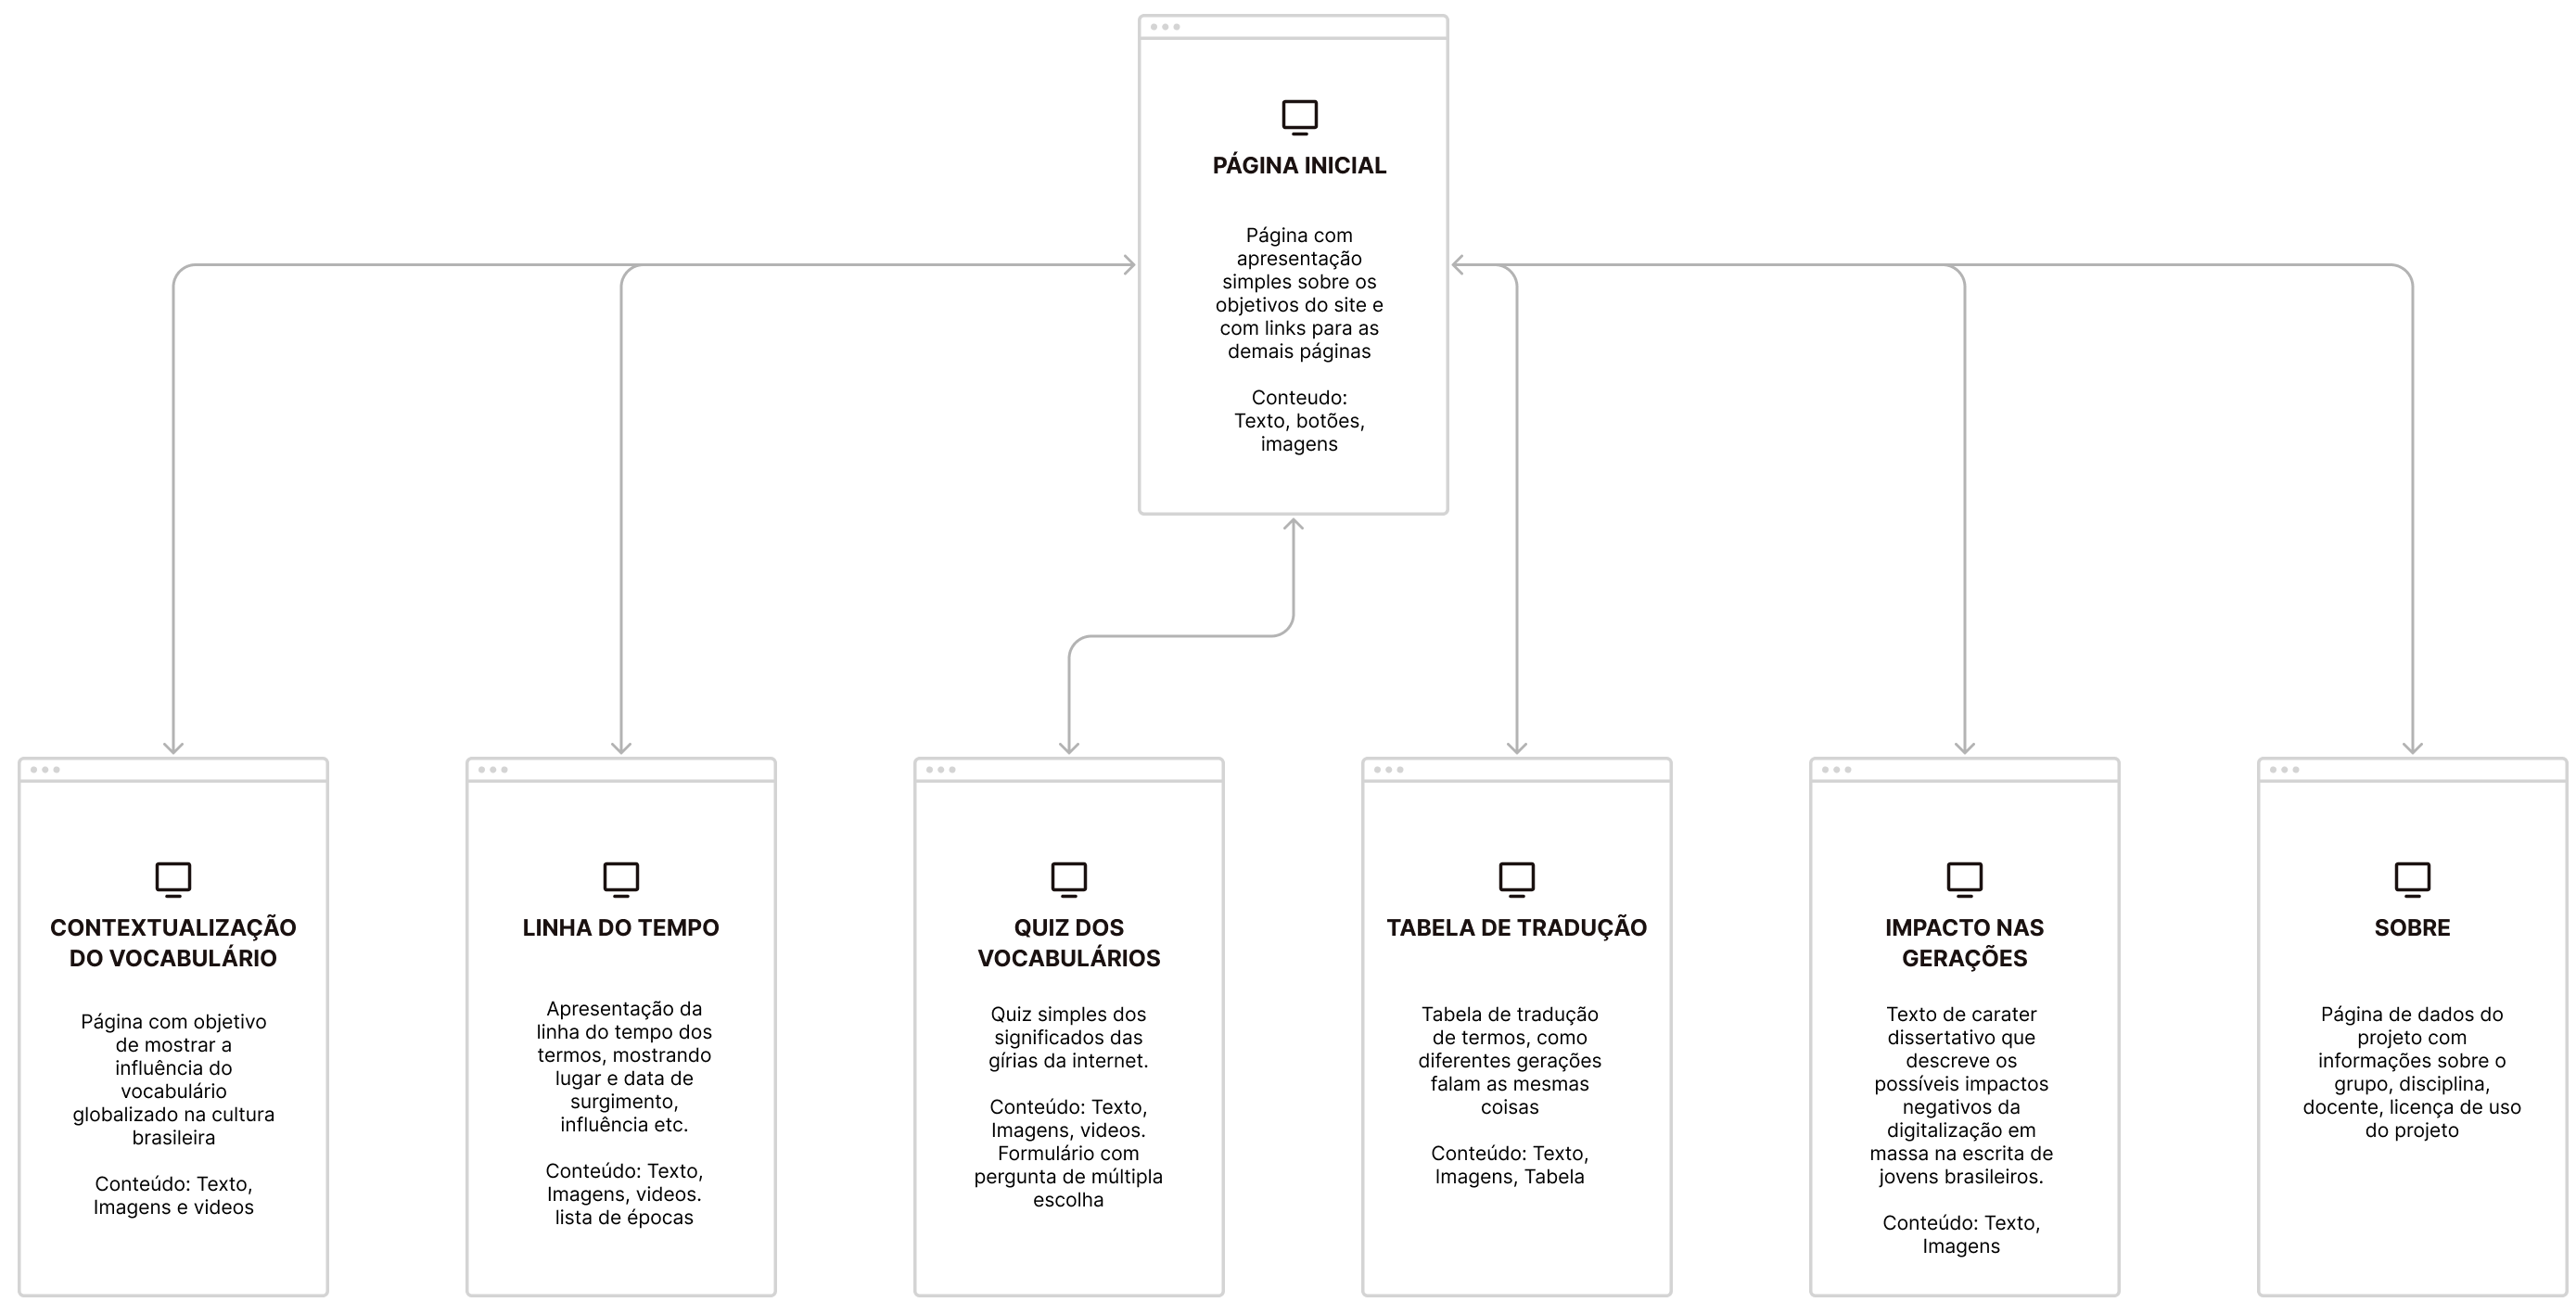
\includegraphics[width=1\textwidth]{Mapa_Web_Site.png}
    \label{fig:mapa_site}
\end{figure}

A Tabela~\ref{tab:mapeamento-arquivos} relaciona cada página do mapa de navegação aos arquivos
HTML, CSS e JavaScript que a implementam, servindo como referência para a localização do código
mencionado ao longo deste relatório.

\begin{table}[H]
\centering
\caption{Mapeamento entre páginas e arquivos do projeto.}
\label{tab:mapeamento-arquivos}
\renewcommand{\arraystretch}{1.35}
\begin{tabular}{>{\raggedright}m{3.2cm} >{\raggedright\arraybackslash}m{9.3cm}}
\toprule
\textbf{Página} & \textbf{Arquivos} \\
\midrule
Página Inicial & \texttt{pagina\_inicial.html} \\
Contextualização do Vocabulário & \texttt{contextualizacao.html} \\
Linha do Tempo & \texttt{linha\_do\_tempo.html}, \texttt{linha\_do\_tempo.css}, \texttt{linha\_do\_tempo.js} \\
Quiz dos Vocabulários & \texttt{quiz\_de\_vocabulario.html} (lógica em JavaScript embutido) \\
Dicionário de Gírias & \texttt{tabela\_de\_traducao.html}, \texttt{dicionario.css}, \texttt{dicionario.js}, \texttt{js/girias\_csv.txt} \\
Impacto nas Gerações & \texttt{impacto\_no\_vocabulario.html} \\
Sobre & \texttt{sobre.html} \\
Base global & \texttt{style.css} (variáveis, componentes e responsividade), \texttt{padrao-comunicacao.svg} \\
\bottomrule
\end{tabular}
\end{table}

A seguir, descreve-se cada seção do mapa de navegação, com seus elementos e comportamentos:

\begin{itemize}[leftmargin=*]
    \item \textbf{Página Inicial:} apresentação sobre os objetivos do site, com \textit{cards}
    de navegação que exibem, nesta entrega final, uma pré-visualização da página de destino ao
    passar o mouse (texto, botões, ícones em SVG e imagens de \textit{preview}).
    \item \textbf{Contextualização do Vocabulário:} página com o objetivo de mostrar a
    influência do vocabulário globalizado na cultura brasileira, por meio de vídeo explicativo
    incorporado e nuvem de palavras interativa, na qual o próprio visitante pode inserir termos
    estrangeiros que usa no cotidiano.
    \item \textbf{Linha do Tempo:} apresentação da linha do tempo dos termos, mostrando lugar e
    data de surgimento e influência, com sistema de zoom progressivo via scroll do mouse e
    controles de zoom/filtro reorganizados em um menu mais compacto nesta entrega.
    \item \textbf{Quiz dos Vocabulários:} quiz interativo sobre os significados das gírias da
    internet, com múltipla escolha, confirmação por questão, bloqueio de alteração após
    confirmar e feedback visual imediato ao usuário.
    \item \textbf{Dicionário de Gírias:} dicionário interativo em formato de livro, com
    paginação animada, busca em tempo real e mais de 100 termos carregados dinamicamente via
    arquivo CSV.
    \item \textbf{Impacto nas Gerações:} texto dissertativo, finalizado nesta entrega, que
    descreve os possíveis impactos da digitalização em massa na escrita de jovens brasileiros,
    acompanhado de bloco de dados estatísticos com referências (texto e imagens).
    \item \textbf{Sobre:} página de dados do projeto, finalizada nesta entrega, com informações
    sobre o grupo, disciplina, docente e licença de uso (texto e tabela).
\end{itemize}

% ─── PROTÓTIPOS VISUAIS E DECISÕES DE INTERFACE ────────────────────────────
\section{Protótipos Visuais e Decisões de Interface}

Esta seção apresenta, para cada página do projeto, a comparação entre o wireframe de baixa
fidelidade concebido na fase de planejamento (à esquerda) e o estado final da implementação
capturado em tela (à direita). Os textos descrevem as decisões tomadas pela equipe ao longo das
sprints e o grau de aderência ao plano original.

Nesta entrega final, além da versão para telas de computador (\textit{desktop}), a equipe também
desenvolveu a \textbf{visão mobile} do site, adaptando a disposição dos elementos, a navegação e
os componentes interativos de cada página para telas menores. Por esse motivo, cada subseção a
seguir traz, além da comparação entre wireframe e versão final em \textit{desktop}, uma captura
de tela adicional da respectiva versão mobile.

% ── Página Inicial ──────────────────────────────────────────────────────────
\subsection{Página Inicial}
\label{sec:protótipos-home}

\begin{figure}[H]
    \centering
    \begin{minipage}[t]{0.38\textwidth}
        \centering
        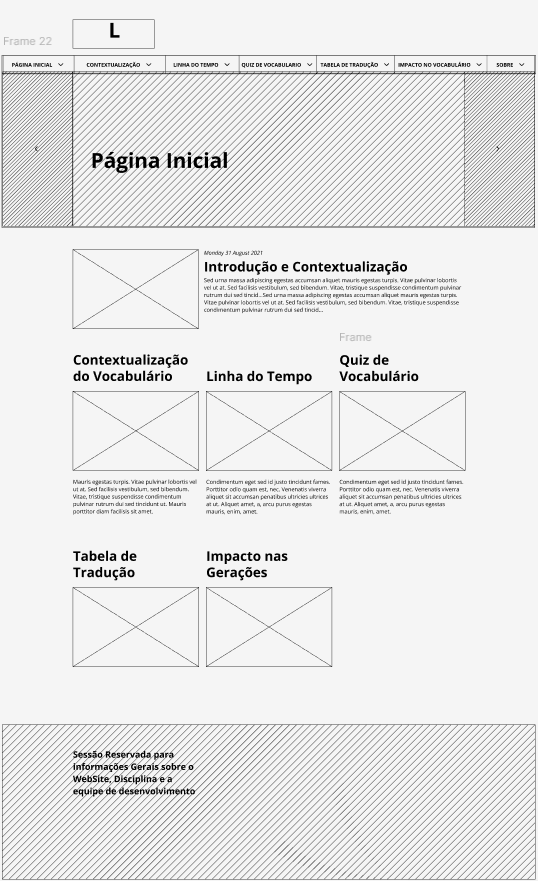
\includegraphics[width=\linewidth]{Pag_1.png}
        \caption*{\textit{Wireframe original}}
    \end{minipage}
    \hfill
    \begin{minipage}[t]{0.57\textwidth}
        \centering
        \includegraphics[width=\linewidth]{PaginaInicial1.png}
        \caption*{\textit{Versão final}}
    \end{minipage}
    \caption{Página Inicial: wireframe planejado e estado final do desenvolvimento.}
    \label{fig:comp_home}
\end{figure}

\begin{figure}[H]
    \centering
    \includegraphics[width=0.35\textwidth]{PaginaInicial1_mobile.png}
    \caption{Página Inicial: versão mobile.}
    \label{fig:mobile_home}
\end{figure}

A estrutura geral segue o wireframe: \textit{hero} com título centralizado, barra de navegação
horizontal e área de conteúdo principal seguida de rodapé informativo. A identidade visual
combinada (paleta verde/dourado, tipografia e padrão SVG de fundo) foi integralmente aplicada. O
principal incremento desta entrega final, não previsto no wireframe original, foi a
implementação dos \textit{cards} de \textit{preview}: ao passar o mouse sobre cada item de
navegação, uma camada de imagem mostra uma amostra real da página de destino, com ícones SVG
substituindo os emojis utilizados anteriormente. O texto introdutório, antes provisório, foi
revisado para refletir o tema da globalização do vocabulário brasileiro.

% ── Contextualização ────────────────────────────────────────────────────────
\subsection{Contextualização do Vocabulário}
\label{sec:protótipos-contexto}

\begin{figure}[H]
    \centering
    \begin{minipage}[t]{0.38\textwidth}
        \centering
        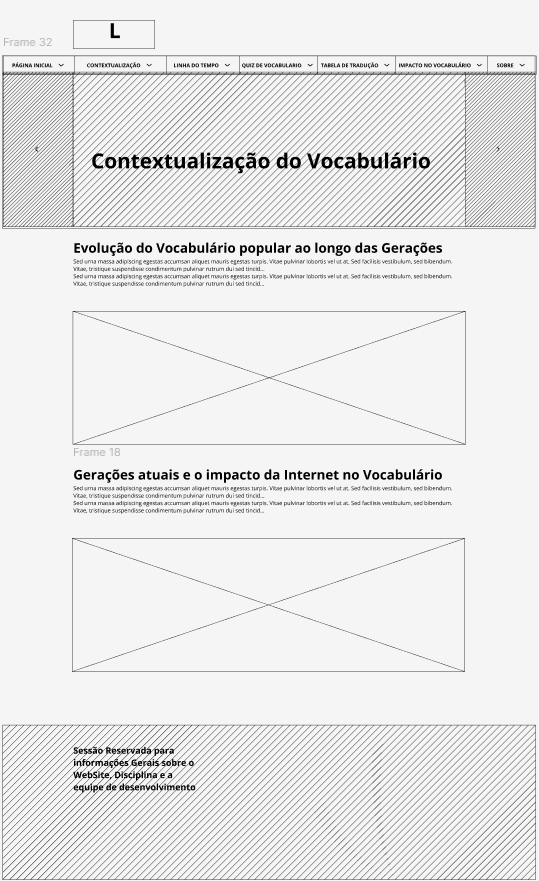
\includegraphics[width=\linewidth]{Pag_2.png}
        \caption*{\textit{Wireframe original}}
    \end{minipage}
    \hfill
    \begin{minipage}[t]{0.57\textwidth}
        \centering
        \includegraphics[width=\linewidth]{Contextualizacao.png}
        \caption*{\textit{Versão final}}
    \end{minipage}
    \caption{Contextualização: wireframe planejado e estado final do desenvolvimento.}
    \label{fig:comp_contexto}
\end{figure}

\begin{figure}[H]
    \centering
    \includegraphics[width=0.35\textwidth]{Contextualizacao_mobile.png}
    \caption{Contextualização: versão mobile.}
    \label{fig:mobile_contexto}
\end{figure}

O wireframe previa dois blocos de texto com imagens estáticas intercaladas. Durante o
desenvolvimento, a equipe optou por uma abordagem mais dinâmica e participativa: o segundo bloco
de imagem foi substituído por uma \textbf{nuvem de palavras interativa}, na qual o próprio
visitante pode inserir termos estrangeiros que usa no cotidiano. Nesta entrega final, o vídeo
explicativo previsto desde o wireframe original foi incorporado à página, e a nuvem de palavras
recebeu o algoritmo de estabilização visual descrito na Seção~\ref{sec:exemplo-nuvem}. Por
recomendação recebida na avaliação por pares,  o vídeo
foi por padrão com autoplay desativado, para melhorar a experiencia do usuario.

% ── Linha do Tempo ──────────────────────────────────────────────────────────
\subsection{Linha do Tempo}

\begin{figure}[H]
    \centering
    \begin{minipage}[t]{0.30\textwidth}
        \centering
        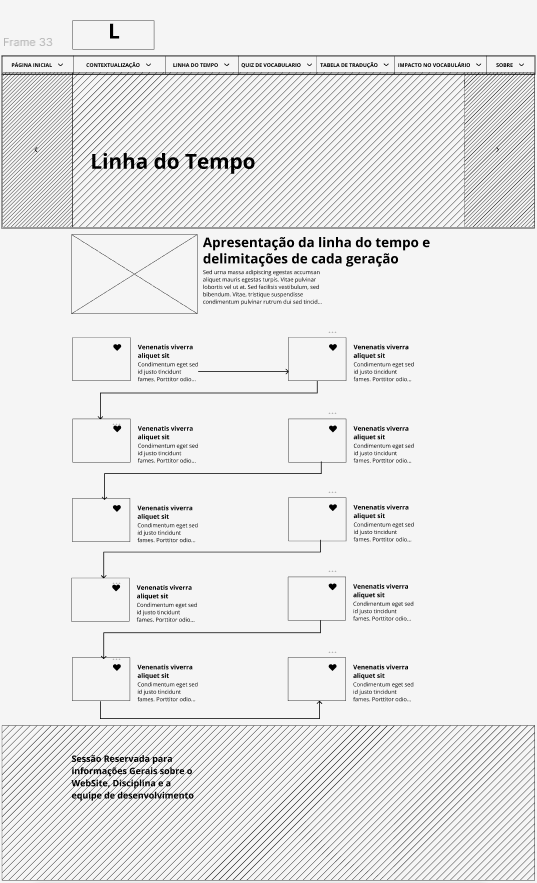
\includegraphics[width=\linewidth]{Pag_3.png}
        \caption*{\textit{Wireframe original}}
    \end{minipage}
    \hfill
    \begin{minipage}[t]{0.57\textwidth}
        \centering
        \includegraphics[width=\linewidth]{LinhaTempo1.png}
        \caption*{\textit{Versão final — visão geral (zoom~0)}}
    \end{minipage}
    \caption{Linha do Tempo: wireframe planejado e estado final em visão geral.}
    \label{fig:comp_timeline1}
\end{figure}

\begin{figure}[H]
    \centering
    \includegraphics[width=0.7\textwidth]{LinhaTempo3.png}
    \caption{Linha do Tempo em zoom máximo (nível~2), revelando eventos detalhados e
    vocabulário associado a cada período.}
    \label{fig:comp_timeline3}
\end{figure}

\begin{figure}[H]
    \centering
    \includegraphics[width=0.35\textwidth]{LinhaTempo1_mobile.png}
    \caption{Linha do Tempo: versão mobile.}
    \label{fig:mobile_timeline}
\end{figure}

Esta página registrou a maior evolução em relação ao wireframe original. O plano inicial previa
uma lista vertical de eventos conectados por setas, uma abordagem diferente, mas ainda estática
e de rolagem longa. A equipe decidiu substituí-la por um \textbf{sistema de zoom progressivo
controlado pelo scroll do mouse}: a visão inicial exibe apenas as três grandes divisões
geracionais (X, Millennials e Z) e, conforme o usuário rola o mouse dentro da área da linha do
tempo, camadas adicionais de detalhes, como eventos específicos, datas e palavras associadas, vão
sendo reveladas progressivamente.

Nesta entrega final, o menu de controles (zoom e filtro por geração) foi reorganizado em um
layout mais compacto, atendendo parcialmente a uma sugestão recebida na avaliação por pares de
separar visualmente o controle de zoom do controle de filtros de época. Os níveis de zoom
continuam controlados pelo atributo \texttt{data-level} de cada evento HTML, conforme descrito na
Seção de exemplos de código HTML.

% ── Quiz de Vocabulário ─────────────────────────────────────────────────────
\subsection{Quiz de Vocabulário}
\label{sec:protótipos-quiz}

\begin{figure}[H]
    \centering
    \begin{minipage}[t]{0.35\textwidth}
        \centering
        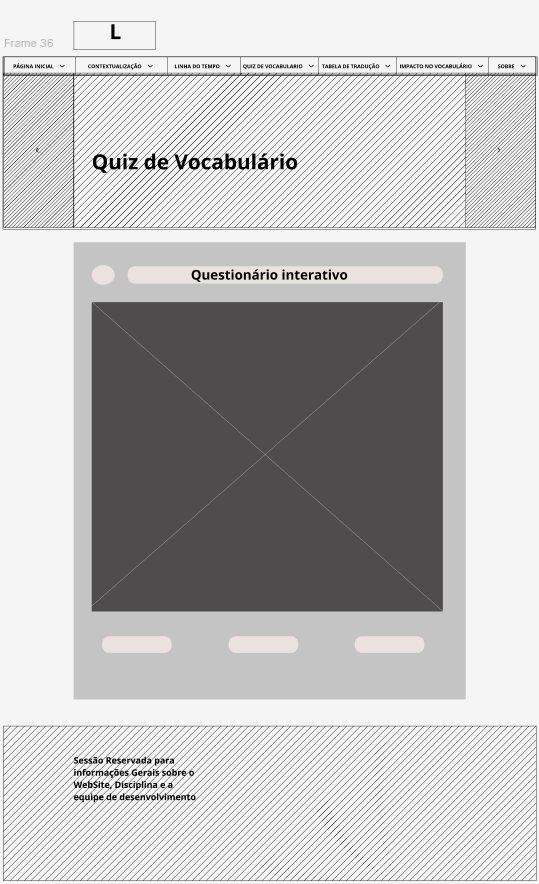
\includegraphics[width=\linewidth]{Pag_4.png}
        \caption*{\textit{Wireframe original}}
    \end{minipage}
    \hfill
    \begin{minipage}[t]{0.60\textwidth}
        \centering
        \includegraphics[width=\linewidth]{Quiz1.png}
        \caption*{\textit{Versão final}}
    \end{minipage}
    \caption{Quiz de Vocabulário: wireframe planejado e versão final implementada.}
    \label{fig:comp_quiz}
\end{figure}

\begin{figure}[H]
    \centering
    \includegraphics[width=0.35\textwidth]{Quiz1_mobile.png}
    \caption{Quiz de Vocabulário: versão mobile.}
    \label{fig:mobile_quiz}
\end{figure}

O wireframe previa um questionário interativo com área de questão central e botões de navegação;
essa estrutura foi mantida na implementação. A versão final traz perguntas de múltipla escolha
com quatro alternativas, confirmação individual por questão e feedback visual imediato (destaque
verde para acerto, vermelho para erro), além do cálculo e exibição do resultado final. A equipe
optou por manter o visual em branco do questionário, priorizando a legibilidade, em vez de
incorporar os tons verde/dourado da identidade do projeto.

% ── Dicionário de Gírias ────────────────────────────────────────────────────
\subsection{Dicionário de Gírias}

\begin{figure}[H]
    \centering
    \begin{minipage}[t]{0.35\textwidth}
        \centering
        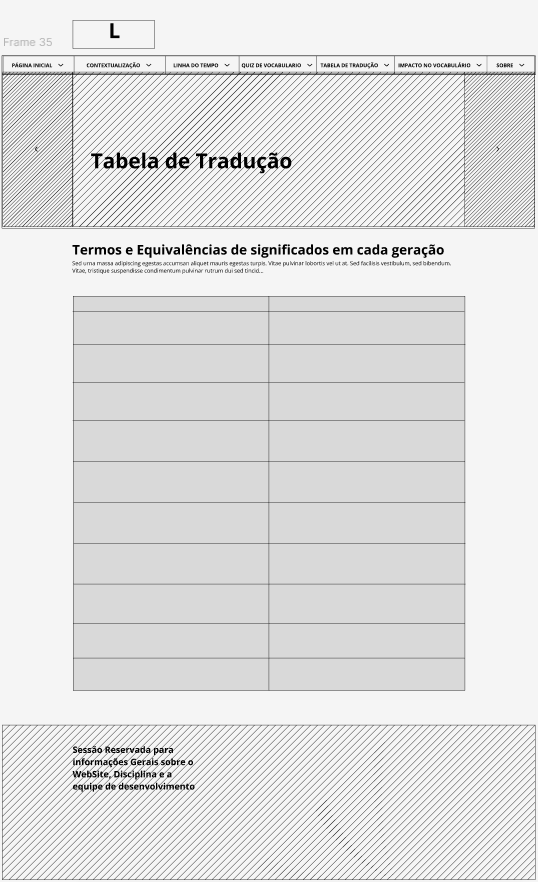
\includegraphics[width=\linewidth]{Pag_5.png}
        \caption*{\textit{Wireframe original — tabela estática}}
    \end{minipage}
    \hfill
    \begin{minipage}[t]{0.60\textwidth}
        \centering
        \includegraphics[width=\linewidth]{Dicionario1.png}
        \caption*{\textit{Versão final — livro interativo}}
    \end{minipage}
    \caption{Dicionário de Gírias: wireframe de tabela estática e versão final em formato de
    livro.}
    \label{fig:comp_dicionario}
\end{figure}

\begin{figure}[H]
    \centering
    \includegraphics[width=0.35\textwidth]{Dicionario1_mobile.png}
    \caption{Dicionário de Gírias: versão mobile.}
    \label{fig:mobile_dicionario}
\end{figure}

Esta página foi a que mais se afastou do wireframe original. O plano inicial previa uma tabela
estática de duas colunas com termos e equivalências. Durante o desenvolvimento, a equipe concluiu
que essa abordagem não transmitia a riqueza do conteúdo nem convidava à exploração. A solução
adotada foi a \textbf{metáfora de livro interativo}: duas páginas lado a lado, com animação CSS de
virada de página, campo de busca em tempo real e paginação completa. O acervo de mais de 100
termos é carregado dinamicamente via arquivo CSV. A avaliação por pares identificou uma
inconsistência no caminho do arquivo CSV referenciado pelo JavaScript; esse ajuste pontual segue
registrado como melhoria a ser corrigida (Seção~\ref{sec:melhorias-futuras}).

% ── Impacto no Vocabulário ──────────────────────────────────────────────────
\subsection{Impacto no Vocabulário}
\label{sec:protótipos-impacto}

\begin{figure}[H]
    \centering
    \begin{minipage}[t]{0.38\textwidth}
        \centering
        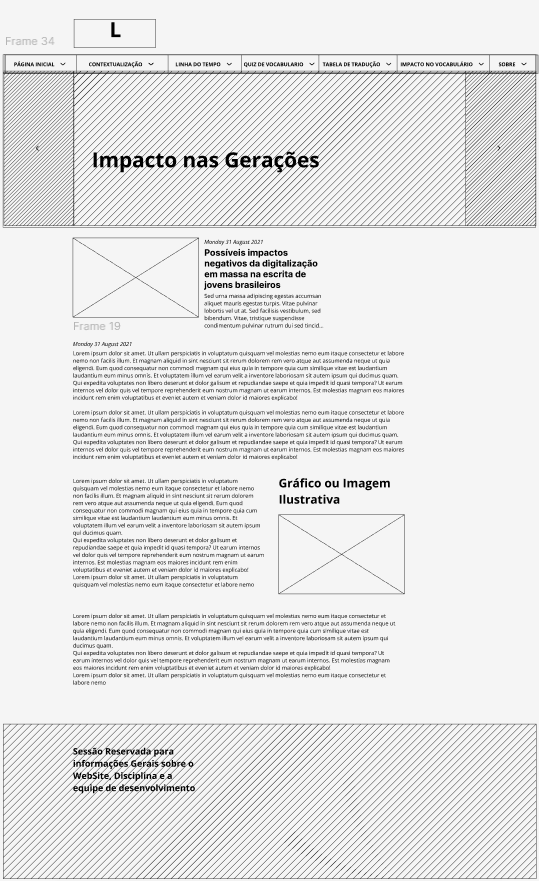
\includegraphics[width=\linewidth]{Pag_6.png}
        \caption*{\textit{Wireframe original}}
    \end{minipage}
    \hfill
    \begin{minipage}[t]{0.57\textwidth}
        \centering
        \includegraphics[width=\linewidth]{Impacto1.png}
        \caption*{\textit{Versão final}}
    \end{minipage}
    \caption{Impacto no Vocabulário: wireframe planejado e estado final do desenvolvimento.}
    \label{fig:comp_impacto}
\end{figure}

\begin{figure}[H]
    \centering
    \includegraphics[width=0.35\textwidth]{Impacto1_mobile.png}
    \caption{Impacto no Vocabulário: versão mobile.}
    \label{fig:mobile_impacto}
\end{figure}

A estrutura visual segue o wireframe: bloco de texto dissertativo com imagem ilustrativa ao lado.
A identidade visual foi aplicada com consistência. Nesta entrega final, o texto definitivo sobre
os impactos da digitalização em massa na escrita dos jovens brasileiros foi redigido por Gustavo
Machado, com reestruturação editorial conduzida por Johnny Sarafim, que organizou um bloco de
dados estatísticos com suas respectivas referências (ver trecho de código na
Seção~\ref{sec:exemplo-html}).

% ── Sobre ───────────────────────────────────────────────────────────────────
\subsection{Sobre}

\begin{figure}[H]
    \centering
    \begin{minipage}[t]{0.38\textwidth}
        \centering
        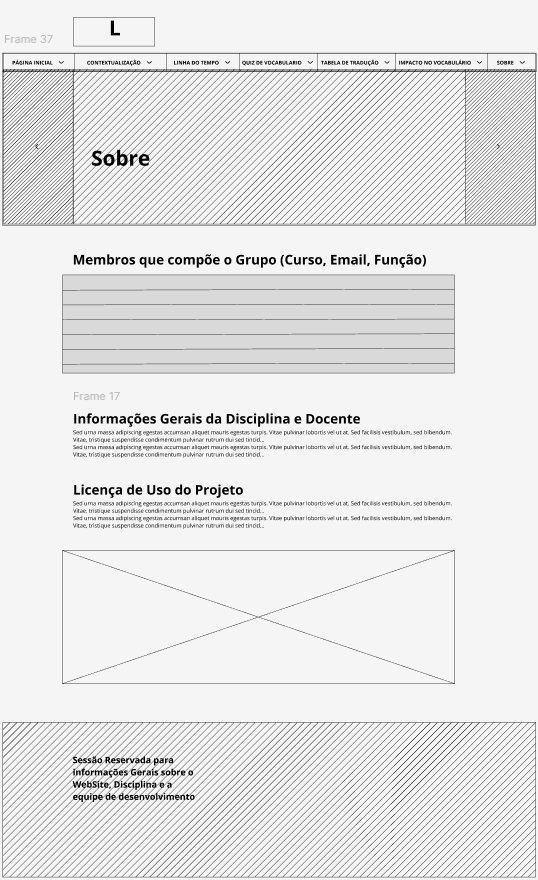
\includegraphics[width=\linewidth]{Pag_7.png}
        \caption*{\textit{Wireframe original}}
    \end{minipage}
    \hfill
    \begin{minipage}[t]{0.57\textwidth}
        \centering
        \includegraphics[width=\linewidth]{Sobre1.png}
        \caption*{\textit{Versão final}}
    \end{minipage}
    \caption{Sobre: wireframe planejado e versão final implementada.}
    \label{fig:comp_sobre}
\end{figure}

\begin{figure}[H]
    \centering
    \includegraphics[width=0.35\textwidth]{Sobre1_mobile.png}
    \caption{Sobre: versão mobile.}
    \label{fig:mobile_sobre}
\end{figure}

A página Sobre foi finalizada nesta entrega, seguindo a estrutura do wireframe: lista de
integrantes, informações gerais da disciplina e docente, e licença de uso. O rodapé padronizado
com os dados do projeto foi implementado de forma consistente em todas as páginas do site.

% ─── MODELO DE LAYOUT CSS ────────────────────────────────────────────────────

\section{Modelo de Layout CSS}

\subsection{Abordagem Geral}

O projeto utiliza uma arquitetura visual baseada majoritariamente em \textbf{Flexbox} e com uma
implementação pontual de \textbf{CSS Grid} para a página da linha do tempo. A estrutura recorrente
é composta por \textit{header} no topo, seção \textit{hero} de destaque, área central de conteúdo
com \texttt{.page-container} e \textit{footer} ao final da página.

As decisões de layout seguem três princípios principais:

\begin{enumerate}[leftmargin=*, label=\roman*.]
    \item \textbf{Consistência:} há uma base comum em \texttt{style.css}, enquanto páginas
    específicas usam folhas complementares, como \texttt{dicionario.css},
    \texttt{linha\_do\_tempo.css} e \texttt{quiz.css};
    \item \textbf{Responsividade:} o comportamento responsivo é definido por \textit{media
    queries} globais e locais (por página), com reorganização da navegação e dos componentes em
    telas menores. Nesta entrega final, esses ajustes foram revisados e ampliados especificamente
    para telas mobile, incluindo a nuvem de palavras da Contextualização e o menu da Linha do
    Tempo;
    \item \textbf{Modularidade:} blocos reutilizáveis como \texttt{.card}, \texttt{.hero},
    \texttt{.page-container} e padrões de botões são reaproveitados em diferentes telas.
\end{enumerate}

\subsection{Variáveis CSS e Paleta de Cores}

A identidade visual é centralizada no seletor \texttt{:root}, com tokens de cor para tons de
verde e dourado, além de variáveis para fundo, texto, borda e sombra.

\begin{lstlisting}[language=CSS, caption={Variáveis CSS globais}]
:root {
    --verde-principal: #2E5E3E;
    --verde-escuro: #1F3F2B;
    --verde-claro: #DDEBDD;

    --dourado-principal: #E9B949;
    --dourado-claro: #F6D98B;
    --dourado-hover: #FFF3D0;

    --fundo-site: #F8F6F0;
    --fundo-card: #FFFFFF;

    --texto-principal: #2B2B2B;
    --texto-secundario: #5F5F5F;
    --texto-claro: #FFFFFF;

    --borda-suave: #D8C89A;
    --sombra-suave: rgba(31, 63, 43, 0.15);
}
\end{lstlisting}

\subsection{Navegação com Flexbox}

A barra de navegação utiliza Flexbox com distribuição uniforme dos links por meio de
\texttt{flex: 1}, mantendo alinhamento central e largura proporcional entre itens.

\begin{lstlisting}[language=CSS, caption={Navegação principal com Flexbox}]
nav {
    width: 100%;
    display: flex;
    background: linear-gradient(90deg, var(--dourado-principal), var(--dourado-claro));
    border-top: 2px solid var(--verde-escuro);
    border-bottom: 2px solid var(--verde-escuro);
}

nav a {
    flex: 1;
    display: flex;
    align-items: center;
    justify-content: center;
    padding: 15px 12px;
    text-decoration: none;
    color: var(--verde-escuro);
    font-size: 12px;
    font-weight: 700;
    text-transform: uppercase;
    border-right: 1px solid rgba(31, 63, 43, 0.35);
    transition: transform 0.25s ease, background 0.25s ease, color 0.25s ease, box-shadow 0.25s ease;
}

nav a:hover {
    background: var(--dourado-hover);
    color: var(--verde-principal);
    transform: scale(1.05);
    box-shadow: 0 6px 14px rgba(31, 63, 43, 0.22);
}
\end{lstlisting}

\subsection{Hero com Background Composto}

A seção \textit{hero} combina camadas de fundo para gerar profundidade visual: sobreposição
escura, padrão SVG repetido e gradiente base.

\begin{lstlisting}[language=CSS, caption={Hero com camadas de background}]
.hero {
    width: 100%;
    height: 220px;
    display: flex;
    align-items: center;
    justify-content: center;
    border-bottom: 3px solid var(--dourado-principal);
    background:
        linear-gradient(
            rgba(31, 63, 43, 0.86),
            rgba(31, 63, 43, 0.86)
        ),
        url("padrao-comunicacao.svg"),
        linear-gradient(135deg, var(--verde-escuro), var(--verde-principal));
    background-size: auto, 400px 238px, auto;
    background-repeat: repeat;
    background-position: center;
}
\end{lstlisting}

\subsection{Layout em Grid na Linha do Tempo}

A Linha do Tempo usa Grid em três colunas para alternância lateral dos cards, com eixo central
reservado para os marcadores.

\begin{lstlisting}[language=CSS, caption={Grid da Linha do Tempo}]
.timeline-event {
    position: relative;
    display: grid;
    grid-template-columns: 1fr 70px 1fr;
    margin-bottom: var(--timeline-gap);
    transition: opacity 0.35s ease, transform 0.35s ease, margin 0.35s ease;
}

.timeline-event:nth-child(odd) .timeline-card {
    grid-column: 1;
    text-align: right;
}

.timeline-event:nth-child(even) .timeline-card {
    grid-column: 3;
    text-align: left;
}
\end{lstlisting}

\subsection{Responsividade com Media Queries}

O projeto combina divisórias globais e específicas por página. No arquivo base, os principais
pontos são 900px e 500px; na página do Dicionário há também ajustes em 1000px e 800px. Nesta
entrega final, esses pontos de quebra foram revisados especificamente para o menu compactado da
Linha do Tempo e para o comportamento mobile geral do site.

\begin{lstlisting}[language=CSS, caption={Media query global em telas menores}]
@media (max-width: 900px) {
    nav {
        flex-direction: column;
    }

    nav a {
        border-right: none;
        border-bottom: 1px solid rgba(31, 63, 43, 0.25);
    }

    .hero h1 {
        font-size: 48px;
        padding: 0 20px;
    }
}
\end{lstlisting}

\section{Exemplos Relevantes de Código CSS}

\subsection{Exemplo 1 — Componente \texttt{.card}}

O componente \texttt{.card} funciona como bloco reutilizável de destaque com borda lateral em
dourado, sombra em duas camadas e elevação no \textit{hover}.

\begin{lstlisting}[language=CSS, caption={Componente card}]
.card {
    height: 100%;
    background: var(--fundo-card);
    padding: 26px;
    border-left: 6px solid var(--dourado-principal);
    border-radius: 8px;
    box-shadow:
        0 3px 10px rgba(0, 0, 0, 0.10),
        0 1px 2px rgba(0, 0, 0, 0.08);
    transition: 0.25s ease;
    border-top: 1px solid rgba(31, 63, 43, 0.10);
    border-right: 1px solid rgba(31, 63, 43, 0.10);
    border-bottom: 1px solid rgba(31, 63, 43, 0.10);
}

.card:hover {
    transform: translateY(-4px);
    box-shadow: 0 8px 20px rgba(31, 63, 43, 0.22);
}
\end{lstlisting}

\subsection{Exemplo 2 — \textit{Preview} de página nos cards da Página Inicial}

A implementação dos \textit{previews}, novidade desta entrega final, utiliza uma camada de
imagem posicionada de forma absoluta sobre toda a área do \textit{card}, exibida apenas no
\textit{hover}. Cada página de destino possui sua própria regra de \texttt{background-image},
combinando uma sobreposição escura semitransparente com a captura de tela real da página.

\begin{lstlisting}[language=CSS,caption={Preview ocupando todo o card e exibindo imagem completa}]
.card-preview {
    position: absolute;
    inset: 0;
    width: 100%;
    height: 100%;
    background-size: 100% 100%, contain;
    background-position: center center, center center;
}

.page-card.preview-impacto .card-preview {
    background-image:
      linear-gradient(rgba(16, 33, 23, 0.16), rgba(16, 33, 23, 0.16)),
      url("../imgs/impacto_vocabulario.png");
    background-repeat: no-repeat, no-repeat;
}
\end{lstlisting}

O uso de \texttt{background-size: 100\% 100\%} para a primeira camada (o gradiente) e
\texttt{contain} para a segunda (a imagem) garante que a sobreposição cubra totalmente o card,
enquanto a captura de tela é exibida sem cortes nem distorção, independentemente da proporção da
imagem original.

\subsection{Exemplo 3 — Animação de virar página no Dicionário}

O visual de livro é reforçado por duas animações distintas de virada: uma para avanço e outra
para retorno.

\begin{lstlisting}[language=CSS, caption={Animação de virada de página}]
.book.flipping-next .right-page {
    animation: pageFlipNext 0.58s ease-in-out;
    transform-origin: left center;
}

.book.flipping-prev .left-page {
    animation: pageFlipPrev 0.58s ease-in-out;
    transform-origin: right center;
}

@keyframes pageFlipNext {
    0% { transform: rotateY(0deg); filter: brightness(1); }
    50% { transform: rotateY(-82deg); filter: brightness(0.92); }
    100% { transform: rotateY(0deg); filter: brightness(1); }
}

@keyframes pageFlipPrev {
    0% { transform: rotateY(0deg); filter: brightness(1); }
    50% { transform: rotateY(82deg); filter: brightness(0.92); }
    100% { transform: rotateY(0deg); filter: brightness(1); }
}
\end{lstlisting}

\section{Exemplos Relevantes de Código HTML}
\label{sec:exemplo-html}

\subsection{Exemplo 1 — Estrutura semântica do Dicionário}

A estrutura da área do livro utiliza elementos semânticos (\texttt{section}, \texttt{article},
\texttt{header}, \texttt{footer}) e regiões com \texttt{aria-label} para navegação assistiva.

\begin{lstlisting}[language=HTML, caption={Estrutura principal do livro}]
<section class="book-stage" aria-label="Livro de girias">

    <button type="button" class="book-arrow book-arrow-left"
            id="prevPage" aria-label="Pagina anterior">‹</button>

    <div class="book" id="dictionaryBook">
        <article class="book-page left-page">
            <header class="page-header">
                <span class="page-kicker">Vocabulario</span>
                <h3 id="leftPageTitle">Girias</h3>
            </header>
            <div class="page-content" id="leftPageContent"></div>
            <footer class="page-footer">
                <span id="leftPageNumber">1</span>
            </footer>
        </article>

        <article class="book-page right-page">
            <header class="page-header">
                <span class="page-kicker">Traducao</span>
                <h3 id="rightPageTitle">Significados</h3>
            </header>
            <div class="page-content" id="rightPageContent"></div>
            <footer class="page-footer">
                <span id="rightPageNumber">2</span>
            </footer>
        </article>
    </div>

    <button type="button" class="book-arrow book-arrow-right"
            id="nextPage" aria-label="Proxima pagina">›</button>

</section>
\end{lstlisting}

\subsection{Exemplo 2 — Marcação de dados na Linha do Tempo}

Cada evento usa \texttt{data-level} e \texttt{data-period} para que o JavaScript filtre por zoom
e por geração.

\begin{lstlisting}[language=HTML, caption={Evento com metadados para filtro}]
<article class="timeline-event major" data-level="0" data-period="millennials">
    <div class="timeline-dot"></div>
    <div class="timeline-card">
        <span class="timeline-year">1981 - 1996</span>
        <h2>Millennials / Geracao Y</h2>
        <p>Primeira geracao a crescer junto com computadores pessoais e internet discada.</p>
    </div>
</article>

<article class="timeline-event detail" data-level="2" data-period="millennials">
    <div class="timeline-dot"></div>
    <div class="timeline-card">
        <span class="timeline-year">1996</span>
        <h2>MSN Messenger e o internetes</h2>
        <span class="word-chip">LOL</span>
        <span class="word-chip">OMG</span>
        <span class="word-chip">AFK</span>
    </div>
</article>
\end{lstlisting}

\subsection{Exemplo 3 — Dados estatísticos na página de Impacto no Vocabulário}

\begin{lstlisting}[language=HTML,caption={Bloco de dados estatísticos na página de impacto}]
<section class="impacto-dados">
  <h3 class="impacto-subtitle">Dados estatísticos...</h3>
  <ul class="impacto-data-list">
    <li>No Brasil, 5,1% da populacao...</li>
    <li>Em pesquisa com 7.088 brasileiros...</li>
  </ul>
</section>
\end{lstlisting}

\section{Exemplos Relevantes de Código JavaScript}

\subsection{Exemplo 1 — Zoom e filtro por período na Linha do Tempo}

A implementação trabalha com estados explícitos (\texttt{zoomAtual}, \texttt{periodoAtual} e
\texttt{scrollBloqueado}). O método \texttt{atualizarLinhaDoTempo} combina os dois critérios de
visibilidade e usa o atributo \texttt{hidden} para controlar exibição.

\begin{lstlisting}[language=JavaScript, caption={Controle de zoom e scroll da Linha do Tempo}]
function atualizarLinhaDoTempo() {
    linhaTempo.dataset.zoom = zoomAtual;

    eventosLinhaTempo.forEach((evento) => {
        const nivelEvento = Number(evento.dataset.level);
        const periodoEvento = evento.dataset.period;

        const visivelPorZoom = nivelEvento <= zoomAtual;
        const visivelPorPeriodo = periodoAtual === "all" || periodoEvento === periodoAtual;

        evento.hidden = !(visivelPorZoom && visivelPorPeriodo);
    });

    rotuloZoom.textContent = textosZoom[zoomAtual];

    botoesPeriodo.forEach((botao) => {
        const ativo = botao.dataset.period === periodoAtual;
        botao.classList.toggle("active", ativo);
    });
}

function lidarComScrollZoom(evento) {
    if (scrollBloqueado) {
        evento.preventDefault();
        return;
    }

    let zoomAlterado = false;

    if (evento.deltaY < 0) {
        zoomAlterado = aumentarZoom();
    } else if (evento.deltaY > 0) {
        zoomAlterado = diminuirZoom();
    }

    if (!zoomAlterado) {
        return;
    }

    evento.preventDefault();
    scrollBloqueado = true;

    setTimeout(() => {
        scrollBloqueado = false;
    }, 450);
}
\end{lstlisting}

\subsection{Exemplo 2 — Algoritmo de estabilização e colisão da Nuvem de Palavras}
\label{sec:exemplo-nuvem}

Tem o papel de garantir que a mesma palavra ocupe sempre uma posição visualmente
estável entre re-renderizações e impedir que as
caixas de texto das palavras se sobreponham na tela.

\begin{lstlisting}[language=JavaScript,caption={Hash determinístico para estabilidade visual da nuvem}]
function gerarHash(texto) {
    let hash = 2166136261 >>> 0;
    for (let i = 0; i < texto.length; i++) {
        hash ^= texto.charCodeAt(i);
        hash = Math.imul(hash, 16777619) >>> 0;
    }
    return hash;
}
\end{lstlisting}


\begin{lstlisting}[language=JavaScript,caption={Detecção de colisão entre caixas de palavras}]
function caixasColidem(caixaA, caixaB) {
    const margem = 6;
    return !(caixaA.x + caixaA.w + margem <= caixaB.x ||
        caixaB.x + caixaB.w + margem <= caixaA.x ||
        caixaA.y + caixaA.h + margem <= caixaB.y ||
        caixaB.y + caixaB.h + margem <= caixaA.y);
}
\end{lstlisting}

Peso visual (tamanho da fonte) de cada palavra é incrementado dinamicamente

\begin{lstlisting}[language=JavaScript,caption={Atualização de pesos e renderização da nuvem}]
        if (pesosUsuario.has(chave)) {
            pesosUsuario.set(chave, Math.min(pesosUsuario.get(chave) + 3, 15));

            const tag = containerTags?.querySelector(`[data-word="${chave}"]`);
            if (tag) {
                tag.style.outline = "2px solid #E9B949";
                setTimeout(() => {
                    tag.style.outline = "";
                }, 600);
            }
        } else {
            const existeNaBase = palavrasBase.some((palavra) => palavra.word.toLowerCase() === chave);
            pesosUsuario.set(chave, existeNaBase ? 3 : 1);

            if (containerTags) {
                criarTagPalavra(valor, chave);
            }
        }

        desenharNuvem();
\end{lstlisting}

\subsection{Exemplo 3 — Estado de seleção e confirmação no Quiz}
\label{sec:exemplo-quiz}

O Quiz mantém dois vetores de estado (\texttt{respostas} e \texttt{confirmadas}) para controlar
navegação e bloqueio de alterações após confirmação, finalizado nesta entrega por Julio Cesar
Navas.

\begin{lstlisting}[language=JavaScript, caption={Navegacao e resultado do Quiz}]
function renderizar() {
    const p = perguntas[indexAtual];

    document.getElementById('contador').textContent =
        (indexAtual + 1) + ' / ' + perguntas.length;

    const lista = document.getElementById('lista-opcoes');
    lista.innerHTML = '';

    p.opcoes.forEach(function(texto, i) {
        const li = document.createElement('li');
        li.classList.add('quiz-opcao');
        li.textContent = texto;

        if (respostas[indexAtual] === i) {
            li.classList.add('selecionada');
        }

        if (confirmadas[indexAtual]) {
            li.classList.add('bloqueada');
            if (i === p.resposta) li.classList.add('correta');
            else if (respostas[indexAtual] === i) li.classList.add('errada');
        }

        li.addEventListener('click', function() {
            if (!confirmadas[indexAtual]) {
                respostas[indexAtual] = i;
                renderizar();
            }
        });

        lista.appendChild(li);
    });
}

function confirmar() {
    if (respostas[indexAtual] === null) {
        alert('Selecione uma alternativa antes de confirmar!');
        return;
    }
    confirmadas[indexAtual] = true;
    renderizar();
}

function mostrarResultado() {
    let acertos = 0;
    for (let i = 0; i < perguntas.length; i++) {
        if (respostas[i] === perguntas[i].resposta) {
            acertos++;
        }
    }

    document.getElementById('tela-pergunta').style.display = 'none';
    document.getElementById('tela-resultado').style.display = 'flex';
    document.getElementById('resultado-pontos').textContent =
        acertos + ' de ' + perguntas.length + ' acertos';
}
\end{lstlisting}

\subsection{Exemplo 4 — Carregamento e parser CSV do Dicionário}

No Dicionário, o carregamento do arquivo e a separação de colunas usam funções dedicadas, com
parser manual para respeitar aspas e ponto e vírgula em campos textuais.

\begin{lstlisting}[language=JavaScript, caption={Carregamento e parser do CSV no Dicionario}]
async function carregarDicionario() {
    try {
        const resposta = await fetch("/js/girias_csv.txt");

        if (!resposta.ok) {
            throw new Error("Nao foi possivel carregar o arquivo girias_csv.txt");
        }

        const textoCsv = await resposta.text();
        termosCompletos = converterCsvParaTermos(textoCsv);
        termosCompletos.sort((a, b) => a.giria.localeCompare(b.giria, "pt-BR"));

        termosFiltrados = [...termosCompletos];
        renderizarLivro();
    } catch (erro) {
        mostrarErroDeCarregamento();
        console.error(erro);
    }
}

function separarColunasCsv(linha) {
    const resultado = [];
    let atual = "";
    let dentroDeAspas = false;

    for (let i = 0; i < linha.length; i++) {
        const caractere = linha[i];
        const proximo = linha[i + 1];

        if (caractere === '"' && proximo === '"') {
            atual += '"';
            i++;
            continue;
        }

        if (caractere === '"') {
            dentroDeAspas = !dentroDeAspas;
            continue;
        }

        if (caractere === ";" && !dentroDeAspas) {
            resultado.push(atual);
            atual = "";
            continue;
        }

        atual += caractere;
    }

    resultado.push(atual);
    return resultado;
}
\end{lstlisting}

% ─── COMPARAÇÃO COM A ORGANIZAÇÃO PREVISTA ─────────────────────────────────
\section{Comparação entre o Planejado e o Realizado (Entrega Final)}
\label{sec:comparacao-final}

\subsection{O que foi planejado}

Desde a Entrega 1, o grupo previu um desenvolvimento incremental em sprints semanais, com papéis
mutáveis e colaboração entre todos os membros. As tarefas foram distribuídas conforme a
Tabela~\ref{tab:sprints}, com foco em estrutura HTML, CSS responsivo, navegação funcional,
catalogação de termos e, na Fase~2, funcionalidades extras, complementação de conteúdo,
acessibilidade e testes finais.

\subsection{O que foi realizado}

A Tabela~\ref{tab:comparacao} compara as entregas previstas com o estado final do projeto.

\begin{table}[H]
\centering
\caption{Comparação entre o planejado e o realizado até a Entrega 3 (versão final).}
\label{tab:comparacao}
\renewcommand{\arraystretch}{1.45}
\begin{tabular}{>{\raggedright}m{3.5cm} >{\raggedright}m{4.5cm} >{\raggedright\arraybackslash}m{4.5cm}}
\toprule
\textbf{Item planejado} & \textbf{Situação prevista} & \textbf{Situação final} \\
\midrule
Estrutura HTML de todas as páginas &
Entregue até a Sprint 2 &
\textcolor{verdeEscuro}{\textbf{Concluído}} — todas as 7 páginas com estrutura semântica
completa \\
\hline
Identidade visual e CSS global &
Entregue até a Sprint 2--3 &
\textcolor{verdeEscuro}{\textbf{Concluído}} — paleta, tipografia e componentes implementados em
\texttt{style.css} \\
\hline
Navegação funcional entre páginas &
Entregue até a Sprint 3 &
\textcolor{verdeEscuro}{\textbf{Concluído}} — barra de navegação responsiva em todas as páginas,
com \textit{cards} de \textit{preview} na Página Inicial \\
\hline
Dicionário de gírias (tabela de tradução) &
Previsto como tabela estática &
\textcolor{verdeEscuro}{\textbf{Superado}} — implementado como dicionário interativo com busca,
paginação e metáfora de livro \\
\hline
Linha do Tempo &
Prevista como lista de épocas &
\textcolor{verdeEscuro}{\textbf{Superado}} — implementada com CSS Grid alternado, zoom em 3
níveis, filtro por geração e menu de controles compactado nesta entrega \\
\hline
Nuvem de palavras (Contextualização) &
Não prevista no wireframe original &
\textcolor{verdeEscuro}{\textbf{Superado}} — algoritmo de \textit{hash} determinístico e
detecção de colisão garantem estabilidade visual (Seção~\ref{sec:exemplo-nuvem}) \\
\hline
Vídeo explicativo (Contextualização) &
Previsto desde o wireframe original &
\textcolor{verdeEscuro}{\textbf{Concluído}} — incorporado nesta entrega final \\
\hline
Conteúdo textual das páginas &
50+ termos e textos de conteúdo redigidos &
\textcolor{orange}{\textbf{Parcialmente concluído}} — texto de Impacto no Vocabulário e página
Sobre finalizados nesta entrega; meta de 50+ termos catalogados não foi formalmente verificada
\\
\hline
Quiz de vocabulário &
Previsto para a Sprint 7 (Fase 2) &
\textcolor{verdeEscuro}{\textbf{Concluído}} — versão final implementada, antecipada e refinada
ao longo de toda a Fase 2 \\
\hline
Responsividade &
Prevista até a Sprint 3 &
\textcolor{verdeEscuro}{\textbf{Concluído}} — \textit{media queries} ampliadas nesta entrega
para o menu da Linha do Tempo e para o comportamento geral em telas mobile \\
\bottomrule
\end{tabular}
\end{table}

\subsection{Desvios e decisões tomadas}

O principal desvio em relação ao planejado, ao longo de todo o semestre, foi positivo: o
Dicionário de Gírias, a Linha do Tempo e a Nuvem de Palavras foram implementados com nível de
interatividade superior ao previsto inicialmente. A decisão de criar um dicionário em formato de
livro com animação CSS, um sistema de zoom baseado em atributos \texttt{data-*} na Linha do
Tempo e um algoritmo próprio de posicionamento estável para a nuvem de palavras surgiu durante o
desenvolvimento, quando a equipe identificou oportunidades de tornar a experiência mais imersiva
e alinhada ao tema do projeto.

O desvio negativo, por outro lado, esteve concentrado no cronograma: como detalhado na
Seção~\ref{sec:aderencia-cronograma}, a produção do conteúdo textual definitivo e a finalização
de páginas como Sobre e Impacto no Vocabulário, originalmente distribuídas ao longo da Fase~2,
terminaram concentradas nas sprints finais, exigindo redistribuição de esforço entre os
integrantes nos últimos dias antes da Entrega 3.

% ─── ESTADO FINAL ──────────────────────────────────────────────────────────────
\section{Estado Final do Desenvolvimento}

Na data desta entrega, o projeto encontra-se com a infraestrutura técnica completa e a totalidade
das funcionalidades planejadas implementadas. O estado final de cada componente é descrito a
seguir:

\begin{itemize}[leftmargin=*]
    \item \textbf{Página Inicial (\texttt{pagina\_inicial.html}):} concluída — estrutura,
    navegação, conteúdo textual introdutório e \textit{cards} de \textit{preview} das demais
    páginas implementados.
    \item \textbf{Contextualização (\texttt{contextualizacao.html}):} concluída — vídeo
    incorporado e nuvem de palavras interativa funcionando com algoritmo de estabilização e
    detecção de colisão.
    \item \textbf{Linha do Tempo (\texttt{linha\_do\_tempo.html} + \texttt{.css} +
    \texttt{.js}):} concluída — eventos de três gerações (X, Millennials e Z), zoom em 3 níveis,
    filtro por período, controle por scroll do mouse e menu de controles compactado.
    \item \textbf{Dicionário de Gírias (\texttt{tabela\_de\_traducao.html} +
    \texttt{dicionario.css} + \texttt{dicionario.js}):} concluída — mais de 100 termos
    carregados via CSV, busca em tempo real, paginação tipo livro e animação de virada de
    página.
    \item \textbf{Quiz de Vocabulário (\texttt{quiz\_de\_vocabulario.html}):} concluída — versão
    final com lógica de seleção, confirmação, navegação entre questões e tela de resultado.
    \item \textbf{Impacto no Vocabulário (\texttt{impacto\_no\_vocabulario.html}):} concluída —
    texto dissertativo definitivo e bloco de dados estatísticos com referências.
    \item \textbf{Sobre (\texttt{sobre.html}):} concluída — informações do grupo, disciplina e
    licença finalizadas.
    \item \textbf{CSS global (\texttt{style.css}):} completo, com variáveis CSS, componentes
    reutilizáveis e responsividade ampliada para telas mobile.
    \item \textbf{Padrão gráfico (\texttt{padrao-comunicacao.svg}):} criado e utilizado no
    \textit{hero} de todas as páginas.
    \item \textbf{Navegação mobile (\texttt{padrao-comunicacao.svg}):} completo, com adaptabilidade e responsividade de
    \textit{hero} de todas as páginas.
\end{itemize}


% ─── CONSIDERAÇÕES FINAIS ────────────────────────────────────────────────────
\section{Considerações Finais}

O projeto chega à Entrega 3 com todas as funcionalidades planejadas implementadas e o conteúdo
textual essencial finalizado, incluindo os itens que se mantinham pendentes na entrega anterior:
\textit{previews} de página na Página Inicial, vídeo e nuvem de palavras finalizada na
Contextualização, Quiz de Vocabulário completo, menu compactado na Linha do Tempo, texto
dissertativo da página de Impacto no Vocabulário, página Sobre e responsividade ampliada para
telas mobile.

Do ponto de vista de processo, no entanto, a equipe reconhece que a abordagem ágil adotada não
conseguiu contemplar corretamente as datas previstas no cronograma original de sprints. Tarefas
de conteúdo foram repetidamente adiadas em favor de funcionalidades de código mais visíveis, e a
ausência de um \textit{product owner} dedicado fez com que esses adiamentos não fossem
formalmente repriorizados sprint a sprint. O resultado foi uma concentração de trabalho nas
últimas semanas antes da Entrega 3, compensada apenas pela mutabilidade dos papéis dentro da
equipe, que permitiu redistribuir esforço para as frentes mais atrasadas no momento certo.

A decisão de investir em componentes interativos de alta qualidade, como o dicionário em formato
de livro, a linha do tempo com zoom progressivo, a nuvem de palavras com posicionamento estável e
o quiz com feedback imediato, resultou em um produto final que demonstra com clareza a proposta
do tema escolhido.

\end{document}